\ifslide{
  \section[Agenda]{}

  \setcounter{tocdepth}{2}

  \begin{frame}
    \begin{multicols}{2}
      \fontsize{7}{8}{
        \tableofcontents[part=1]

      }
    \end{multicols}
  \end{frame}
  \part{Introduction au Middleware}
}

\ifbook{
  \chapter{Le Middleware}
}

\section{A - Rappel} % (09/01/2012)}

\abstractframe{En introduction au cours, une suite de rappels et de définitions sont effectués dans
ce chapitre. Cette démarche assure la mise en place d'une sémantique et d'une terminologie commune. En
outre, lors du parcours des rappels et des prérequis, une intention particulière est portée sur les
éléments qui seront essentiels de retenir pour les prochains chapitres.}
{../img/overview.png}

\mysubsection{Fonctionnement d'un ordinateur}

\ifbook{

  \mysubsubsection{Fonctionnement schématique d'un ordinateur}

  \paragraph{} Avant d'entrer dans le coeur du sujet, il est nécessaire de tout d'abord bien
  comprendre comment fonctionne la brique la plus élémentaire de tout système informatique:
  l'ordinateur.

  \begin{figure}[hb]
    \begin{center}
      \includegraphics[scale=0.3]{img/cpu-schematics.png}
      \caption{Schéma simplifié du fonctionnement d'un ordinateur}
      \label{schema-ordi}
    \end{center}
  \end{figure}

  \paragraph{} Comme l'illustre le dessin \ref{schema-ordi} (page \pageref{schema-ordi}), un
  ordinateur, aussi complexe soit-il peut être résumé aux trois composants suivants:
  \begin{description}
    \item[Processeur] unité de traitement de l'ordinateur, c'est lui qui réalise les calculs et qui
    produit les résultats.
    \item[Mémoire] espace de travail du processeur, la mémoire lui permet de placer les résultats,
    intermédiaires ou finaux, de ses calculs
    \item[Entrées/Sorties] pour communiquer avec le "monde extérieur" (clavier, écran, disques durs,
    réseaux,...) l'ordinateur dispose de différents composant matériels dédiés aux différentes
    entrées/sorties avec qui il interagit.
  \end{description}

  \paragraph{Distinction mémoire vive et mémoire morte} Sans rentrer dans les détails techniques, il
  est important de noter que les périphériques de stockage, tels que les disques durs,
  ne sont pas conceptuellement très différents de la mémoire. Dans les deux cas, ils permettent au
  processeur de stocker des résultats.

  \paragraph{} Ce qui sépare donc ces deux composants est leur \textbf{persistance}. L'information
  située en mémoire est \textbf{volatile}, elle disparaît si l'ordinateur s'éteint brusquement. À
  l'inverse, les données placées sur un périphérique de stockage, persiste au-delà de l'extinction de
  l'ordinateur.
}

\ifslide{
  \begin{frame}{Qu'est-ce qu'un ordinateur ?}
   \begin{center}
     \includegraphics[scale=0.3]{img/cpu-schematics.png}
   \end{center}
  \end{frame}
}

\ifbook{
    \mysubsubsection{Rôle du système d'exploitation}

    \paragraph{} Encore une fois de manière très schématique, et surtout en restant pertinent par
    rapport au thème du cours, le \textit{Middleware}, nous allons maintenant brièvement évoquer le
    rôle du système d'exploitation.

    \paragraph{} En repartant de ce que nous venons de détailler sur le fonctionnement d'un
    ordinateur, plusieurs points peuvent rapidement être gênants. Le principal est que le processeur
    n'exécute qu'un seul programme à la fois, donc tel quel, seule une application peut s'exécuter
    sur un ordinateur.

    \paragraph{} Le système d'exploitation est une couche logicielle qui va permettre aux programmes
    s'exécutant sur l'ordinateur de se partager les ressources mises à disposition par l'ordinateur
    (processeur, mémoire, périphériques de stockage,...). En outre, le système d'exploitation va
    jouer le rôle d'arbitre entre ses différents programmes, leur attribuant, chacun à leur tour, un
    certain temps d'utilisation de ces ressources.

    \paragraph{} Ainsi, c'est grâce aux systèmes d'exploitation que de multiples programmes vont
    pouvoir s'exécuter en \textbf{parallèle} sur une machine, qu'elle possède un ou plusieurs
    processeurs.

    \paragraph{} Il est important de noter qu'aucun ordinateur ne pourra effectuer plus de tâches en
    parallèle que son nombre de processeurs, mais les cycles d'exécutions étant extrêmement rapides,
    un seul ordinateur, équipé d'un seul processeur, peut donner l'impression à son utilisateur
    d'exécuter simultanément plusieurs tâches. C'est l'impression que vous donne tous les jours,
    les ordinateurs dédiés à la bureautique que vous utilisez.

    \paragraph{Remarque} On notera aussi au passage qu'un même programme peut lui même se diviser en
    plusieurs processus distincts, s'exécutant aussi en parallèle, selon les règles évoquées juste
    avant. Ainsi, dans la cadre d'un projet \textit{middleware} la question de l'exécution, de
    manière concurrente, de différentes parties de l'application peut se poser... (Nous y
    reviendrons plus loin dans le cours).

    \paragraph{} Le schéma \ref{role-os} (page \pageref{role-os} résume les principales
    fonctionnalités d'un système d'exploitation vis-à-vis des applications qui s'exécutent en son
    sein.

    \begin{figure}[h]
      \begin{center}
        \includegraphics[scale=0.3]{img/operating-system.png}
        \caption{Rôle du système d'exploitation}
        \label{role-os}
      \end{center}
    \end{figure}
}

\ifslide{
  \begin{frame}{Le rôle du système d'exploitation}
    \begin{center}
      \includegraphics[scale=0.3]{img/operating-system.png}
    \end{center}
  \end{frame}
}

\ifbook{
  \mysubsubsection{Limites physiques d'un ordinateur}
  \paragraph{} Avant d'aller plus loin, arrêtons-nous un instant sur ces notions et sur le système,
  aussi schématique soit-il que nous venons de décrire. Au regard de son fonctionnement, quelles
  limites pouvons-nous déjà percevoir ? Dans quelles conditions, un tel système - l'ordinateur, aura
  des difficultés à effectuer les opérations qu'on lui confie ?

  \paragraph{} Sans surprise, on peut distinguer à peu près autant de limites que de composants
  distingués dans la précédente représentation. Etudions, sommairement, pour chacun d'entre eux les
  limites qu'ils induisent sur l'ordinateur.

  \paragraph{Processeur} La première limite physique d'un ordinateur, qui est pratiquement
  incontournable, est le processeur. Un processeur peut effectuer un certain nombre d'opérations
  dans un certain délai. Dans un système parfaitement optimisé, où tous les autres - assez
  nombreux, nous allons le voir, goulots d'étranglement ont été "neutralisés", cette vitesse
  d'exécution est une limite incompressible : l'ordinateur ne pourra simplement exécuter les
  opérations demandées plus rapidement...

  \paragraph{Parallélisme} Comme évoqué lors de la description du rôle d'un système d'exploitation,
  un ordinateur exécute souvent plusieurs processus à la fois, souvent plus nombreux que son nombre
  de processeurs. Ainsi, il doit passer d'un processus à un autre, à tour de rôle, pour permettre à
  tous de s'exécuter \textit{presque} en parallèle.

  \paragraph{} Il est évident que le passage d'un processus à un autre n'est pas gratuit, et nécessite, de
  la part du système d'exploitation, comme du processeur, un travail supplémentaire qui consiste à
  sauvegarder les données et l'état du processus placé en "pause" et à recharger ceux du processus
  qui "reprend la main".

  \paragraph{} Au bout du compte, si l'ordinateur effectue un nombre de tâches en parallèle
  largement trop grand pour sa capacité, il risque de passer plus de temps à \textbf{changer de
  contexte} entre chaque processus, plutôt qu'à réellement effectuer les opérations qu'on lui
  demande.

  \paragraph{Mémoire} La mémoire à la disposition du processeur impacte généralement grandement la
  vitesse d'exécution. En effet, plus l'ordinateur pourra placer de données en mémoire, plus il
  pourra avoir à sa disposition des résultats intermédiaire et finaux.

  \paragraph{} Illustrons rapidement ce point par un exemple concret. Supposons que l'on confie à
  l'ordinateur de trier un tableau de données, composé d'une seule colonne, par ordre de grandeur
  croissante du contenu de chaque cellule

  \begin{figure}[h]
    \begin{center}
      \includegraphics[scale=0.3]{img/exemple-algo.png}
      \caption{Algorithme de tri avec une case mémoire}
      \label{algo-exemple}
    \end{center}
  \end{figure}

}

\ifslide{

  \begin{frame}{Exemple d'algorithme}
    \begin{center}
      \includegraphics[scale=0.3]{img/exemple-algo.png}
    \end{center}
  \end{frame}
}

\ifbook{
  \paragraph{} Si l'ordinateur ne peut stocker qu'un seul résultat intermédiaire, en l'occurrence la
  taille du contenu de la cellule, il ne peut réordonner le tableau qu'en échangeant les cellules
  de positons. En effet, il peut calculer la taille d'une cellule, la stocker, calculer la taille de
  la seconde cellule, la comparer à la précédente et changer l'ordre des deux cellules, si
  nécessaire, puis continuer...

  \paragraph{} Après un laborieux travail, cet \textbf{algorithme}, illustré sur la figure
  \ref{algo-exemple}  (page \pageref{algo-exemple}), sera donc capable de réordonner l'ensemble du
  tableau, mais en effectuant un important nombre de calculs. À l'inverse, si le processeur est
  libre de placer autant de résultats en mémoire que d'entrées dans le tableau, il pourra se
  contenter de calculer, une fois pour toute, la taille de chaque cellule, puis de les trier de
  manière plus "globale"...

  \paragraph{Remarque} Cet exemple est volontairement très grossier et n'est pas représentatif du
  tout du fonctionnement interne réel d'un ordinateur, ni même de la manière dont le processeur va
  implémenter un algorithme de tri. Néanmoins, sans être l'exemple le plus respectueux des détails
  techniques d'un ordinateur, il illustre de manière très juste l'importance de la mémoire pour la
  réalisation d'opérations au sein d'un ordinateur.

  \paragraph{Entrées/Sorties} Après la mémoire, c'est très certainement les entrées/sorties la
  source de goulot d'étranglement la plus commune au sein d'un ordinateur. Pour bien comprendre
  l'impact de ces dernières sur les performances de l'ordinateur, il suffit de regarder la figure
  \ref{pyramid-io} (page \pageref{pyramid-io} qui décrit, sous forme de pyramide, la vitesse d'accès
  des différentes entrées/sorties, les unes par à rapport aux autres.

  \begin{figure}[h]
    \begin{center}
      \includegraphics[scale=0.3]{img/pyramid-io.png}
      \caption{Vitesse des entrées/sorties selon les périphériques}
      \label{pyramid-io}
    \end{center}
  \end{figure}

}

\ifslide{
  \begin{frame}{Vitesse d'accès des périphériques}
    \begin{center}
      \includegraphics[scale=0.3]{img/pyramid-io.png}
    \end{center}
  \end{frame}
}

\ifbook{

  \paragraph{} À l'étude de ce tableau, il apparait assez flagrant que si une information nécessaire
  à la bonne exécution du programme est située sur un périphérique inutilement lent (par exemple: sur
  disque dur plutôt qu'en mémoire, sur un serveur distant plutôt que sur le disque dur,...), le
  système en sera ralenti.

  \paragraph{Remarque:} \textit{Ce développement sur les limites physiques d'un ordinateur est volontaire.
  En effet, dans le cadre de la conduite de projet \textit{Middleware}, ces limites seront à
  prendre à compte, dès la conception et l'architecture d'une solution logicielle, pour s'assurer que,
  lors de sa mise en production, le système construit ait une chance de donner les performances
  souhaitées.}

  \paragraph{}\textit{Si des experts techniques sont généralement là pour assister les personnes en charge
  de la conduite, il reste important que ces dernières gardent ses problématiques à l'esprit et soient
  capables d'en discuter avec les sus-nommés experts...}

}

\newpage
\mysubsection{Du modèle client/serveur aux applications "web"}

\ifbook{
  \mysubsubsection{Bref histoire du client léger}
  \paragraph{} Avec l'apparition des réseaux informatiques, apportés par des technologies telles que
  TCP/IP sur laquelle s'est construit le désormais célèbre protocole HTTP, il est rapidement apparu
  très intéressant de pouvoir répartir le traitement sur plusieurs machines.

  \paragraph{} En effet, au début de l'informatique, les machines puissantes coûtaient relativement
  cher, et avaient des capacités de calcul permettant d'effectuer des calculs complexes et de
  répondre aux besoins de nombreux utilisateurs. Ainsi est né le modèle client/serveur, où
  l'utilisateur, à l'aide d'un terminal - une machine peu puissante et peu coûteuse de comme le minitel
   - se connecte à une machine lui servant des données et exécutant les traitements demandés - un serveur.
  Le terminal se contentant, dans ce modèle, d'afficher le résultat.

  \begin{figure}[h]
    \begin{center}
      \includegraphics[scale=0.3]{img/mainframe-terminals.png}
      \caption{Terminaux et mainframe}
      \label{mainframe}
    \end{center}
  \end{figure}
}

\ifslide{
  \begin{frame}{Mainframe et terminaux}
    \begin{center}
      \includegraphics[scale=0.3]{img/mainframe-terminals.png}
    \end{center}
  \end{frame}
}

\ifbook{

  \paragraph{} Avant d'aller plus loin, on peut noter avec intérêt que ce modèle n'est en fin de
  compte pas très différent de celui des débuts d'internet. En effet, à leurs débuts, les
  navigateurs "web" (Mozaic, Netscape, puis Internet Explorer) se contentaient simplement d'afficher le
  contenu des pages HTML qu'on leur servait. Nous y reviendrons par la suite...

  \mysubsubsection{La naissance du client "lourd"}

  \paragraph{} Ce premier modèle client/serveur se construisait donc sur deux logiciels distincts,
  une première partie s'exécutant sur le terminal de l'utilisateur, le \textbf{client léger}, et une
  seconde partie, plus élaborée et embarquant la \textbf{logique métier} de l'application, le
  \textbf{serveur}.

  \paragraph{Remarque} \textit{L'usage a malheureusement imposé depuis longtemps l'utilisation du même
  terme, \textit{serveur} pour désigner deux entités conceptuellement similaire, mais concrètement
  différentes. Ce terme peut en effet indiquer une machine physique, un ordinateur, relié à un
  réseau informatique et utilisé, à distance, par des utilisateurs, mais aussi le logiciel s'exécutant
  sur ce même type d'ordinateur et fournissant un service applicatif à ces mêmes utilisateurs.}

  \paragraph{} \textit{La différence est relativement aisée à saisir, mais elle peut tout de même
  prêter à confusion. Si dans le cas de la partie précédente nous évoquions le concept de machine
  physique, dans cette section, nous parlons très clairement de \textbf{serveur logiciel}.}

  \paragraph{} Alors que la puissance à la disposition des terminaux augmentait, et que, dans les
  faits, ceux-ci devinrent des ordinateurs graphiques à usage personnel ("\textit{Personal Computer
  (PC)}"), il apparut rapidement très pertinent d'en profiter pour offrir des clients plus puissants,
  capable d'effectuer des traitements par eux-mêmes, et donc offrir des fonctionnalités
  supplémentaires à leur utilisateurs.

  \paragraph{} Ainsi le mouvement de balancier, qui avait pour but de placer le maximum de logique
  applicative et de traitement du côté du \textit{serveur}, s'est inversé et les logiciels clients
  devinrent à leur tour de plus en plus complexe, au point qu'on les qualifia de \textbf{clients
  lourds}.

  \begin{figure}[h]
    \begin{center}
      \includegraphics[scale=0.3]{img/fat-clients.png}
      \caption{L'arrivée du PC et des clients lourds}
      \label{fat-clients}
    \end{center}
  \end{figure}

  \mysubsubsection{Les limites du modèle}

  \paragraph{} Si cette nouvelle déclinaison du modèle aboutit clairement à une meilleure productivité
  des utilisateurs, du moins dans la plupart des cas, elle posa aussi rapidement des problématiques
  complexes en terme de maintenance. En effet, pour pouvoir faire évoluer le logiciel, il faut
  désormais modifier à la fois le client et à la fois le serveur, et assurer leur redéploiement
  synchrone. On se retrouva vite malheureusement dans des situations difficiles à gérer, où de
  multiples versions d'une même application clientes étaient déployées et devaient cohabiter avec des
  versions différentes de leurs serveurs...
}

\ifslide {
  \begin{frame}{Le modèle client/serveur}
    \begin{center}
      \includegraphics[scale=0.3]{img/fat-clients.png}
    \end{center}
  \end{frame}
}


\mysubsection{La persistance des données}
\ifslide {
  \begin{frame}{La persistance}
    \begin{center}
      \includegraphics[scale=0.3]{img/persistance.png}
    \end{center}
  \end{frame}
}

\ifbook{
  \mysubsubsection{La Persistance des données: du fichier à la base de données}
  % fichier et répertoires
  \paragraph{} Avant de voir comment les technologies de type client/serveur ont évolué pour
  circonvenir les problématiques apparues avec l'émergence du client lourd, intéressons-nous un instant
  non plus au logiciel, mais à ses données, et surtout à leur persistance.

  \paragraph{} Comme évoqué plus haut, un ordinateur travaille avec des données en mémoire qui
  sont donc par essence, \textbf{volatiles}. En effet, lors de l'interruption de l'alimentation de la
  mémoire, les données qu'elle contient sont purement et simplement perdues. Les données n'étant,
  dans la plupart des applications, que rarement dispensables, il a été impératif de trouver des
  mécanismes pour assurer leur \textbf{persistance}.

  \paragraph{} L'unité atomatique de cette persistance est le \textbf{fichier}. Cette abstraction
  permet de sauvegarder sur une unité de stockage (en langage vernaculaire, un "disque dur") un ensemble
  d'information de manière séquentielle. On peut retrouver les informations stockées à l'aide du nom
  du fichier.

  \paragraph{} En fait, on peut aisément comparer un fichier à une simple feuille, sur laquelle on
  écrit les données que l'on souhaite voir persister, un peu de la même manière dont on écrit sur une
  feuille sa liste de courses, pour justement, ne pas l'oublier.

  \paragraph{} Pour permettre de trier et de ranger ses fichiers, dans la prolongation de l'image
  choisie pour les fichiers, des fichiers spéciaux, les \textbf{répertoires} ont été conçu pour
  permettre de ranger aisément et hiérarchiquement ces fichiers.

  \paragraph{} Malheureusement, la manière séquentielle d'organiser les informations d'un fichier
  se révéla contraignante. En effet, alors que les applications se complexifiaient, et qu'une donnée
  fit référence à une autre, puis à une autre, la nature \textbf{relationnelle} devint évidente et
  imposa un changement de stratégie dans l'approche de leur persistance.

  \paragraph{} En outre, les données nécessitent bien souvent d'être partagées entre plusieurs
  applications, et il est fort complexe de partager un fichier de données entre plusieurs
  applications. Comment gérer les accès concurrents ? Comment assurer la cohérence des données qui
  ont été persistées ?
  % base de donnée
  \paragraph{} Pour palier à ces nombreux problèmes et surtout clairement séparer les données des
  applicatifs, les premières bases de données relationnelles firent leur apparition. En plus de
  permettre de stocker les données hors des applications et de les partager, elles permirent, peu à
  peu, d'établir un langage standard pour interagir avec elles, le SQL (\textit{Standard Query
  Language}).
}

\ifslide{
  \demoframe{Le SQL}{
    \begin{center}
      \begin{block}{Une rapide démonstration du langage SQL...}
        \begin{itemize}
          \item les reqêtes de type SELECT
          \item les mise à jour avec UPDATE
          \item Jointure et requête avancée
          \item limite de la portabilité de SQL
        \end{itemize}
      \end{block}
    \end{center}
  }
}
\ifbook{
  \mysubsubsection{Architecture n-tiers}
    \paragraph{} Si nous résumons les différents éléments évoqués jusqu'à maintenant sous forme de
    la figure \ref{n-tiers} (page \pageref{n-tiers}), on constate que désormais notre application,
    qui au départ s'exécutait sur une seule machine, reliée par un terminal très primaire, est
    désormais réellement éclatée entre plusieurs composants, ou \textbf{tiers}.

    \paragraph{} Ainsi, de l'architecture client/serveur, composé de deux tiers, on est arrivé à une
    architecture 3 tiers, où la base de données vint s'ajouter, en tant que troisième tiers. Mais en
    fait, la séparation des fonctions sur différentes instances physiques a continué, et
    aujourd'hui on parle plus en plus souvent d'architecture \textbf{n-tiers}.

    \begin{figure}[h]
      \begin{center}
        \includegraphics[scale=0.3]{img/n-tiers.png}
        \caption{Exemple d'architecture n-tiers}
        \label{n-tiers}
      \end{center}
    \end{figure}
}

\ifslide{
  \begin{frame}{Architecture n-tiers}
    \begin{center}
      \includegraphics[scale=0.35]{img/n-tiers.png}
    \end{center}
  \end{frame}
}

\ifbook{
  \mysubsubsection{Le Web}
  \paragraph{} Avec l'arrivée des technologies du "Web", soit essentiellement au début HTML et HTTP,
  le mouvement de balancier évoqué dans une précédente section s'inverse de nouveau. Dans leurs
  laboratoires, les concepteurs initiaux de ce protocole de communication visèrent avant tout la
  simplicité pour assurer surtout une bonne compatibilité entre les différents systèmes existants
  de part le monde.

  \paragraph{} En effet, avant d'aller plus loin, il est important de se rappeler que à cette
  époque, il existait de nombreux systèmes d'exploitation, tous différents et rarement interopérables
  entre eux. Les plus connus aujourd'hui sont Apple et Windows, mais à l'époque s'ajoutaient aussi de
  nombreux types d'Unix différents (cf. \textit{\mylink{http://en.wikipedia.org/wiki/Unix\_wars}{Unix
  Wars}}), accompagnés par de nombreux autres systèmes, tel que OpenVMS.

  \paragraph{} Sans compter que ces systèmes avaient même des protocoles de communications
  différents. Pour reprendre l'exemple de OpenVMS, ce système utilisait un protocole propriétaire à
  son constructeur, intitulé DecNet et non le standard \textit{de facto} d'aujourd'hui, le protocole
  TCP/IP.

  \paragraph{} Ainsi, concevoir un système applicatif portable - c'est à dire qui fonctionnerait à
  peu près partout et permettrait de communiquer aisément entre des systèmes différents n'était pas
  une simple tâche. C'est donc en partie pour ces raisons, que les concepteurs de HTTP et de HTML
  ont choisi de faire très simple.

  \paragraph{} Le protocole en lui-même est un simple protocole \textbf{texte}, et non binaire, il
  est donc aisé de l'implémenter et, au besoin, de regarder l'échange en lui même pour comprendre la
  source d'un problème. Comme les données échangées sont du texte, tout système de l'époque, aussi
  différent soit-il des autres, était capable de le comprendre.
}

\ifslide{
  \demoframe{Le protocole HTTP}{
    \begin{block}{Démonstrations}
      \begin{itemize}
        \item simple connection avec telnet
        \item connection complète avec les \textit{Developers tools} de Google Chrome
      \end{itemize}
    \end{block}

    \begin{center}
      \includegraphics[scale=0.5]{img/telnet-google.png}
    \end{center}
  }
}

\ifbook{

  \paragraph{} Toujours par souci de simplicité, l'objectif était dans les faits assez peu ambitieux,
  puisqu'il s'agissait d'afficher du contenu simple, du texte un peu enrichi, pour permettre en fait
  au milieu universitaire de publier, facilement et rapidement,  à l'intention de leurs confrères,
  des informations.

  \paragraph{} La conséquence directe de ce choix simple de données utilisées à été de limiter le
  rôle du client à afficher, du mieux possible selon le système utilisée, les informations
  fournies par le serveur HTTP. Le \textbf{client lourd} venait de faire un régime et redevenait un
  \textbf{client léger}.

  \begin{figure}[h]
    \begin{center}
      \includegraphics[scale=0.3]{img/internet.png}
      \caption{Extrait de code HTML contenant du Javascript et du CSS}
      \label{internet}
    \end{center}
  \end{figure}
}

\ifslide {
  \begin{frame}{Le "Web"}
    \begin{center}
      \includegraphics[scale=0.3]{img/internet.png}
    \end{center}
  \end{frame}
}

\ifbook{
  \mysubsubsection{Les technologies "Web" s'enrichissent}
  \mysubsubsubsection{Formulaire et session HTTP}

  \paragraph{} Le protocole HTTP, et son format de données, HTML, a eu le succès qu'on connaît, et
  rapidement, malgré l'élégance de la simplicité de la solution, il apparut clair que l'\textbf{absence
  d'interaction} entre l'utilisateur et le serveur HTTP était une limite trop contraignante. En
  effet, tel que nous l'avons évoqué jusqu'à maintenant, le modèle ne permet en essence que de
  télécharger une page au contenu \textbf{statique}.

  \paragraph{} Pour introduire plus d'interactivité, et permettre au serveur HTTP de modifier
  \textbf{dynamiquement} le contenu des pages présentées selon les demandes des utilisateurs, les
  formulaires ont été introduits. Ces derniers, associés à la méthode HTTP POST, ont donc permis aux
  utilisateurs d'envoyer des données au serveur HTTP, qui furent le point de départ des premières
  applications "web".

  \paragraph{} Mais une fois qu'il fût possible d'envoyer ces données, d'autres limites firent leurs
  apparitions. La plupart des applications nécessitant souvent plusieurs échanges entre l'utilisateur
  et le serveur, il fut nécessaire d'ajouter un mécanisme de son côté pour lui permettre de
  conserver les données associées à l'utilisateur, ou plutôt à sa \textbf{session}.

% TODO:Cookies ?
%  \paragraph{} DPL: Le protocole HTTP est un protocole d'échange de page et sans notion de session.
%  Le cookie a été utilisé pour palier à ce manque.
%  L'ajout donc de la notion de session HTTP permit, là encore, de contourner les limites
%  du modèle original, mais elle ne suffit pas entièrement. De la même manière dont le serveur avait
%  besoin de garder trace de son utilisateur, il fallait aussi que l'on soit en mesure, coté client,
%  de conserver une trace.

  \mysubsubsubsection{CSS et Javascript}
  \paragraph{} Alors que la première génération de site web finissait de fleurir, une
  problématique, jusque là invisible, apparut de plus en plus clairement. Le HTML, dans toute la
  beauté de sa simplicité, enfreint par son essence même, une règle pourtant fondamentale de
  l'informatique, que nous avons déjà évoqué avec les bases de données : la séparation du contenu et de
  sa présentation.

  \begin{figure}[h]
    \begin{center}
      \includegraphics[scale=0.3]{img/html-code-sample.png}
      \caption{Extrait de code HTML contenant du Javascript et du CSS}
      \label{middleware}
    \end{center}
  \end{figure}
}


\ifslide {
  \begin{frame}{HTML, CSS et JavaScript}
    \begin{center}
      \includegraphics[scale=0.3]{img/html-code-sample.png}
    \end{center}
  \end{frame}
}

\ifbook{
  \paragraph{} En effet, au sein d'une page HTML, on mélange avec allégresse texte avec sa
  présentation qu'il s'agisse de le mettre en gras ou en italique, ou bien de le positionner au sein de la
  page. Et cet état de fait a rendu rapidement très difficile de faire évoluer, du point fonctionnel, les sites -
  puisque les graphistes ou ergonomes ne pouvaient pas travailler de manière indépendante des
  programmeurs, mais aussi de faire évoluer leurs chartes graphiques, puisque leur simple mise à
  jour nécessitait de modifier l'intégralité des pages...

  \paragraph{} C'est ainsi qu'est apparu le CSS, \textit{Cascading Style Sheet}, ou plus
  simplement, les feuilles de styles, dont l'objectif était non seulement de permettre de modifier
  la présentation d'une page HTML existante, mais aussi de séparer la partie présentation d'un site,
  de ses données.

  \paragraph{} En parallèle à l'utilisation du CSS, un autre langage a été introduit, sous forme de
  scripts, placés dans la page, mais dont l'exécution est déclenchée par le navigateur et qui donc
  fonctionne non plus sur le serveur, mais sur le poste client.

  \paragraph{} Introduit tout d'abord de manière propriétaire, ce petit langage permit de rendre les
  sites "web" tellement plus dynamiques et \textbf{conviviaux}, en améliorant grandement
  l'interaction de l'utilisateur avec ces derniers, qu'il fut rapidement adopté, et même normalisé
  sous le nom, rarement utilisé, de ECMAScript.
}

\ifbook {
  \mysubsubsection{Conteneur d'exécution d'application}
  \paragraph{} Comme nous l'avons brièvement résumé, les technologies du "web" se sont construites
  sur une forte volonté d'offrir un système ouvert, standard et interopérable. À l'aide des
  abstractions choisies, et du modèle relativement simple, une page HTML, aussi complexe soit-elle,
  peut être rendue - à peu près, de manière similaire, quelque soit le système d'exploitation
  utilisé.

  \paragraph{} Mais, du coté serveur, les technologies étaient toujours très \textbf{adhérentes} à ce
  dernier. Que vous exécutiez sur Apache HTTP, à l'aide du mod CGI, des scripts Shell sous Unix, ou
  que vous écriviez des pages ASP sur un serveur Microsoft, le code réalisé restait indéniablement
  spécifique à son cadre d'exécution.

  \paragraph{} Progressivement, un certain nombres de cadre d'exécution (et de développements)
  d'application "web" virent le jour, tel que PHP et Java. Ces deux derniers, pour continuer avec
  eux, forment des langages de programmation à part entière, mais le modèle qu'ils proposent apporte
  surtout une réelle interopérabilité coté serveur.

  \paragraph{} En effet, avec ce genre de technologie, il devint possible d'exécuter son programme
  sur n'importe quel type de serveur avec un comportement (presque) identique. On put donc enfin
  aisément migrer de systèmes d'exploitation, dans le cas où celui-ci ne se comporte pas de manière
  suffisante pour l'application, ou recruter un développeur sans que celui-ci n'ai besoin d'autres
  compétences que la seule maîtrise de la technologie.

  \paragraph{} En outre, ces technologies promeuvent, pour la plupart, un certain \textbf{modèle de
  programmation}, et l'écosystème qui les entoure apporte son lot de composants prêts à utiliser
  et destinés à faciliter grandement le développement d'applications "web" robustes et capables de
  monter en charge.

  \begin{figure}[h]
    \begin{center}
      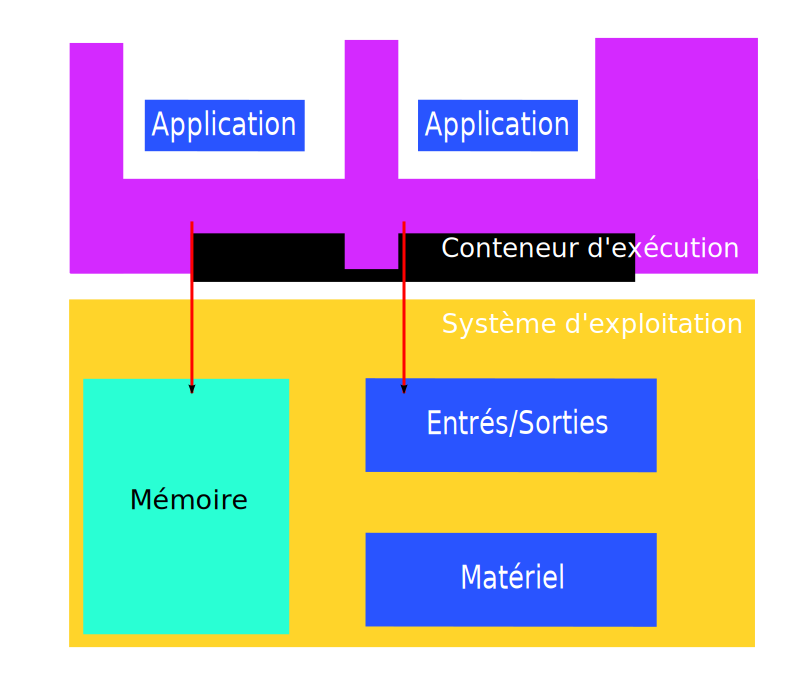
\includegraphics[scale=0.3]{img/execution-container.png}
      \caption{Rôle d'un conteneur d'exécution}
      \label{execution-container}
    \end{center}
  \end{figure}
}


\ifslide {
  \begin{frame}{Conteneur d'exécution}
    \begin{center}
      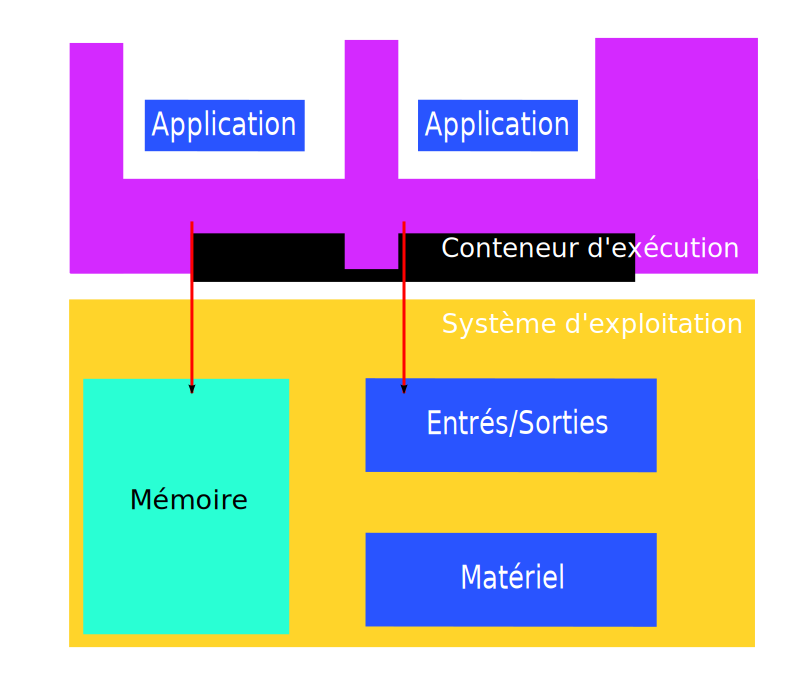
\includegraphics[scale=0.3]{img/execution-container.png}
    \end{center}
  \end{frame}
}

\newpage
\mysubsection{Qu'est ce que le middleware ?}

\ifbook {
  \paragraph{} Après ce vaste état des lieux, nous allons enfin pouvoir rentrer dans le thème de ce
  cours: le \textit{Middleware}. En premier lieu, essayons de trouver une définition un plus parlante
  de ce terme, qui n'a pas réellement de traduction française.

  \paragraph{} Si l'on traduit très littéralement ce terme, on obtient quelque chose de l'ordre du
  "matériel du milieu". Bon, c'est peu parlant, mais clairement le suffixe "\textit{-ware}" fait echo
  aux termes \textit{"software"} - le matériel logiciel, et \textit{"hardware"}, le matériel
  physique, ce qui signifie que, en fait, le mot clé ici, est le "milieu".

  \paragraph{} Mais de quoi exactement sommes-nous au milieu ici ? Revoyons simplement notre dessin
  d'architecture à n-tiers:

  \begin{figure}[h]
    \begin{center}
      \includegraphics[scale=0.3]{img/n-tiers.png}
      \caption{Où se trouve le middleware sur cette figure ?}
      \label{where-is-middleware}
    \end{center}
  \end{figure}
}

\ifslide{
   \begin{frame}{Qu'est ce que le middleware ?}
     \begin{center}
       \includegraphics[scale=0.35]{img/n-tiers.png}
     \end{center}
   \end{frame}
}

\ifbook{

  \paragraph{} Le \textit{Middleware} est tout simplement ce qui se retrouve, littéralement, au
  milieu ! Soit entre la base de données et les clients utilisées par les usagers du système. Mais
  au milieu, il y a l'application, non ? Certes oui, mais, celle ci ne s'appuie désormais plus sur les
  seules API fournies par le système d'exploitation, mais sur une kyrielle de services. Ces derniers
  proviennent soit de son environnement d'exécution - tel que une machine virtuelle comme celle de
  Java ou C\#, ou un serveur d'application, ou encore par des composants que l'application elle-même
  embarque.

  \paragraph{} Mais qu'apportent ces services de plus ? Nous allons étudier le "catalogue" en
  détails durant ce cours, mais en quelques mots, ils apportent beaucoup ! Gestion de \textit{pool}
  de connexion, cache locale ou distribué, sécurité, intégration avec un service d'authentification
  distant ou même encore la capacité de mettre en \textit{cluster} l'application pour assurer
  aisément sa montée en charge simplement en ajoutant de nouvelles machines.

  \paragraph{} Pour en revenir à une sorte de définition du \textit{Middleware}, nous retiendrons
  donc que ce dernier est l'ensemble des services utilisées par l'application, aussi bien en son
  sein, que pour communiquer avec des services distants. Bref, en essence, le \textit{Middleware} se
  trouve bel et bien "au milieu", entre l'application et le reste du monde...

  \paragraph{} En essence, le \textit{Middleware}, c'est les briques avec lesquelles on construit
  l'application métier que l'on souhaite réaliser.
  % TODO: dessin fin de déf du middleware: reprendre l'img de plomberie du bootcamp
}

\subsection{Caractéristiques de la Programmation Orienté Objet}

\newcommand{\bizProcessExemple}[0]{
  \begin{enumerate}
    \item créer un nouveau salarié dans la base de données
    \item ajouter la salarié dans l'équipe de son manager
    \item notifier par email les membres de l'équipe de l'arrivée du nouveau membre
  \end{enumerate}
}

\ifbook{

  \paragraph{} La paradigme de la programmation orienté objet se retrouve dans  plusieurs
  problématiques liées au \textbf{Middleware}, il est important d'expliciter quelques unes de ses
  caractéristiques.

  \subsection{Programmation impérative}

  \paragraph{} La paradigme de la programmation orienté objet se retrouve dans  plusieurs
  problématiques liées au \textbf{Middleware}, il est important d'expliciter quelques unes de ses
  caractéristiques.

  \paragraph{} En premier lieu, il faut savoir que la programmation orienté object se définit
  essentiellement par sa distinction avec la programmation \textbf{procédurale} ou
  \textbf{impérative}. Dans ce style de programmation, on effectue les traitements les uns à la suite
  des autres, en regroupant le code commun dans des fonctions.

  \paragraph{} Prenons l'exemple de traitement procédurale:

  \bizProcessExemple

  \paragraph{} Une approche impérative consisterait ici à réaliser un programme réalisant chacune de
  ces actions, dans l'ordres. C'est une approche tout à fait valide et elle ne pose pas, en soi, de
  problème.

  \subsection{Approche par "objet"}

  \paragraph{} Néanmoins, la programmation orienté objet propose une approche, qui apporte de nombreux
  avantages. Cette approche consiste à ne plus se concentrer sur la séquence de traitement à réaliser,
  mais plutôt sur les données utilisées.

  \paragraph{} En effet, le but du jeu ici est d'\textbf{encapsuler} les données dans des objets, et
  ne le laisse le reste du programme interagir avec ces données que par le biais des fonctions
  qu'elles proposent. Ces fonctiones se nomment en fait désormais des \textbf{méthodes}.

  \paragraph{} L'objectif de ceci est de \textbf{masquer} la nature réelle des données, et de
  n'exposer que les traitements disponibles autour de ces données. Ainsi, si la nature des données ou
  même des détails d'implémentations des traitements proposés venaient à changer, ces modifications
  seront transparente pour le reste du programme.
}

\ifslide {
  \subsection{Programmation impérative versus programmation orienté objet}
  \begin{frame}
    \begin{block}{Ajout d'un nouvel employé}
      \bizProcessExemple
    \end{block}
    \begin{center}
      \includegraphics[scale=0.30]{img/biz-process-banner.png}
    \end{center}
  \end{frame}
}

\ifbook{

  \paragraph{} Illustrons ce point en reprenant notre exemple précédent. Pour implémenter notre
  processus métier - l'ajout d'un nouveau employé dans une équipe, nous allons désormais définir
  plusieurs \textbf{objet}.

  \paragraph{} Le premier objet sera l'objet salarié. Ce dernier résultura de la création du salarié
  dans la base de données de l'entreprise, et il regroupe l'ensemble des données relatives à un
  employé. L'accès à la base de données des salariés sera aussi un objet.

  \paragraph{} Le second objet sera en fait une collection de salarié que forme son équipe. Pour
  réaliser le second point de notre traitement, il suffira donc d'ajouter le salarié créée juste avant
  à la liste des salariés composant l'équipe.

  \paragraph{} Un autre objet sera en charge de l'envoi des mails, et sera donc utilisé pour notifier
  les différents membres de l'équipe de l'arrivée du nouveau membre de l'équipe.
}

\ifslide{
  \begin{frame}
    \begin{center}
      \includegraphics[scale=0.25]{img/biz-process-code-sample.png}
    \end{center}
  \end{frame}
}

\ifbook{

  \begin{figure}[h]
    \begin{center}
      \includegraphics[scale=0.3]{img/biz-process-code-sample.png}
      \caption{Exemple de code orienté objet}
      \label{biz-process-code}
    \end{center}
  \end{figure}

  \paragraph{} Comme l'illustre l'extrait de code \ref{biz-process-code} (page
  \pageref{biz-process-code}, ce style de programmation qu'est la  programmation orienté objet
  permet d'obtenir un code très simple et lisible, mais surtout facilement réutilisable. Par
  exemple, l'objet DataAccessObject regroupe tout le code nécessaire pour se connecter à la base de
  données. Il suffit de réutiliser cet objet, ailleurs dans le code du programme si l'on souhaite
  effectuer des opérations avec la base de données.

  \paragraph{} Un autre avantage immédiat de cette approche est de pouvoir concevoir aisément des
  objets "métiers" décrivant de manière isolé et unitaire, les différents traitements spécifique au
  métier de l'entreprise ou l'organisation. Les différents applications pourront ensuite aisément
  s'appuyer sur ces bibliothèques d'objets pour réaliser les différents traitements qui leur sont
  spécifiques.
}

%- dessin "application" => "pile, gestion de threads, cache, ...", puis vers le modèle java/jee de container
%- évoqué la problématique du packaging et de la réutilisation de code, probablématique de gestion de version aussi

% expliciter/décrire le besoin, dans la conception d'un IT, de découper son "business" en module,
% d'avoir est du code partagé (des Jars) mais aussi des applicatifs qui utilisent les mêmes briques,
% les mêmes services, etc...


\section{B - Les services applicatifs 1/2 (10/01/2012)}

\abstractframe{Ciblé sur application, ce chapitre du cours se concentre
sur les services et composants proposés par les \textit{middlewares} à cette
dernière}{../img/overview-services.png}

\ifbook {
  \mysubsection{Remarque préliminaires}
  \paragraph{} \textit{Le champ d'expertise de l'auteur de ce document est Java/JEE, et plus spécifiquement,
  les produits JBoss. Cet état de fait n'est pas sans conséquence sur le contenu du cours, qui
  s'appuye souvent des composants logicielle spécifique à Java.}

  \paragraph{} \textit{Ainsi, bien que la plupart des concepts évoqués dans cette partie se retrouvent
  généralement, sous une forme ou une autre, dans d'autres univers technologique, certains seront
  néanmoins parfois relativement spécifique à l'univers Java ou au monde JBoss.}

  \paragraph{} \textit{Dans la mesure du possible, lorsque ces cas seront évoqués, leur spécifités sera
  soulignés. Le lecteur devra tout de même rester vigilant...}

}

\mysubsection{Conteneur d'exécution virtuelle}

\ifbook {
  \mysubsubsection{Difficultés des applications natives}

  \paragraph{} Reprenons là où nous avons arrêté, dans le section précédente, la description d'un
  serveur. Nous avions donc une machine physique ou virtuelle dont les resources (mémoire,
  entrées/sorties, processeurs) sont partagé par l'intermédiaire du système d'exploitation, qui joue
  le rôle d'arbitre entre les différentes applications.

  \paragraph{} Si ce modèle fonctionne très bien, et de nombreuses applications très efficase ont été
  réalisée sans couche d'abstraction supplémentaire, il pose néanmoins quelques problèmes. Tout
  d'abord, même si l'application utilise le système d'exploitation pour manipuler ressources et sous
  processus, son exécution peut toujours mettre en péril le bon fonctionnement de l'ensemble du
  système.

  \paragraph{} En effet, une application \textbf{native} - qui signifie, dans notre contexte, qu'elle
  n'utilise que les primitives offertes par le système d'exploitation, peut toujours rendre le système
  inopérant en allouant trop de mémoire, en créant trop de sous processus ou encore en écrivant
  beaucoup trop de donnés sur disque.

  \paragraph{} En outre, si les primitives offertes par le système d'exploitation permet au
  développeur de facilement allouer de la mémoire pour son programme, il reste à sa charge de
  s'assurer que cette espace mémoire soit bien libéré dès qu'il n'est plus utilisé.

  \paragraph{} De prime abord, ceci peut sembler trivial, mais c'est en fait très complexe, et
  beaucoup de programme native ont souvent des \textbf{fuites mémoires} qui pose de grave problème
  de performance lors de l'exécution du programme, ou qui, pire encore, entraine le \textit{crash} du
  programme lors de son utilisation.

  \paragraph{} Mais comment se font ces fuites mémoires ? Simplement lorsque le ou les développeurs
  ont oubliés, quelque part au sein de l'application, de libérer des resources. Il peut s'agit par
  exemple. Ainsi, la mémoire reste alloué, tout le temps, et plus le programme s'exécute, plus ils
  "bloque" de la mémoire, jusqu'à atteindre un point où le système d'exploitation ne lui permet plus
  d'en allouer de nouveau.

}
% TODO: slide fuite mémoire

\mysubsection{L'arrivée des conteneurs d'exécution}

\ifslide{
  \begin{frame}{Garbage collection}
   \begin{center}
     \includegraphics[scale=0.3]{img/garbage-collection.jpg}
   \end{center}
  \end{frame}
}

\ifbook{
  \mysubsubsection{"Garbage collection"}
  \paragraph{} Rapidement la gestion de la mémoire est devenu un tel frein au développement
  d'application, que de nombreuses recherches et expérimentations ont été entreprise pour construire
  une sorte de "méta application" qui assurerait la libération de la mémoire, simplifiant ainsi
  grandement la charge du développeur.

  \paragraph{} Ce \textbf{conteneur d'exécution\footnote{Le terme \textbf{conteneur d'exécution
  virtuelle} est une traduction somme toute très personnelle du terme anglais \textit{runtime
  container}. L'usage a imposé de désigne ce genre de container par leur nom (ex: JVM), plutôt que par
  un terme générique, comme système d'exploitation.}} se charge donc garder traces de toute
  allocations mémoires, mais aussi du nombre de référence vers ces dernières. Lorsque il n'existe
  plus, au sein, du programme, de référence vers un espace mémoire allouée, il ne reste plus qu'à
  faire le \textbf{nettoyage}. En anglais, on emploi fréquement le terme de \textit{\textbf{Garbage
  Collection}}.

  \mysubsubsubsection{Libération de la mémoire}
  \paragraph{} Comme toujours la création de ce nouveau \textbf{contexte d'exécution} a aussi été une
  opportunité d'introduire une nouvelle couche d'abstraction permettant au programme de se détacher du
  système d'exploitation.

  \paragraph{} Ainsi, on ne développe plus un programme à l'aide des primitives offertes par tel ou
  tel système d'exploitation, mais à l'aide de celles offertes par son conteneur d'exécution. Charge à
  ce conteneur de s'assurer du fonctionnement idoine de ces primitives quelques soit le système
  d'exploitation sur lequel il s'exécute.

  \mysubsubsection{Quelques conteneurs d'exécution}
  \paragraph{} La machine virtuelle Java est un exemple de tel conteneur d'exécution, mais aussi
  l'intépréteur python on PHP. Ces différents programmes exécutent un code, qu'il soit compilé ou non
  avant\footnote{C'est d'ailleurs cette seule notion de code compilé ou interprété qui distingue
  principalement la machine virtuelle Java des interpréteurs comme Python}, en abstrayant le système
  d'exploitation sous jacent.

  \begin{figure}[hb]
    \begin{center}
      \includegraphics[scale=0.3]{img/sample-containers.png}
      \caption{Quelques conteneurs d'exécution le plus utilisé}
      \label{interop}
    \end{center}
  \end{figure}
}

\ifslide{
  \begin{frame}{Quelques conteneurs d'exécution}
   \begin{center}
     \includegraphics[scale=0.3]{img/sample-containers.png}
   \end{center}
  \end{frame}
}

\ifbook{
  \paragraph{} Si les conteneurs d'exécution abstrait le programe du système d'exploitation sur
  lequel il s'exécute, il est donc ainsi possible d'écrire un même programme Java ou un script
  Python de telle manière qu'il s'exécute de manière similaire sur différents système d'exploitation.

  \paragraph{} Attention néanmoins, si cette \textbf{interopérabilité} est rendue possible par
  l'utilisation d'un conteneur d'exécution, il faut néanmoins prendre soin de l'assurer lors de la
  conception du programme. En effet, on peut toujours aisément rendre son code très adhérant aux systèmes
  d'exploitation utilisé, et ceci malgré l'abstraction offerte par le conteneur.

  \paragraph{} Un exemple très concret de ce dernier point est l'utilisation de chemin de fichier
  spécifique à Windows©, plutôt que d'utiliser des URLs ou un chemin de fichier standard:

  \begin{figure}[hb]
    \begin{center}
      \includegraphics[scale=0.3]{img/interop.png}
      \caption{Exemple de problématique de portabilité au sein d'un conteneur}
      \label{interop}
    \end{center}
  \end{figure}
}

\ifslide{
  \begin{frame}{Interopérabilité}
   \begin{center}
     \includegraphics[scale=0.25]{img/interop.png}
   \end{center}
  \end{frame}
}

\ifbook{
  \paragraph{} C'est donc à propos des applications développées sur ces nouveaux conteneurs
  d'exécutions, et non plus de manière \textbf{native}, que nous allons désormais discuté. On
  notera, au passage, que, au bout du compte, ces conteneurs d'exécutions forment un premier
  \textbf{Middleware} pour l'application.
}

\mysubsection{Serveur d'applications}

\ifbook{

  \paragraph{} À l'aide des conteneurs précédemment évoqués, nous avons maintenant un cadre robuste et
  portable d'exécution de programme, nous offrant déjà des primitives relatives élaborés. Néanmoins,
  ces contextes d'exécutions sont toujours conçu pour exécuter un seul programme. Certes, ce programme
  peut créer des sous processus, mais en essence, le conteneur n'est pas conçu pour exécuter
  différentes applications de manière concurrente.

  \paragraph{} Nous allons voir apparaitre la notion de \textbf{serveur d'applications} - avec un 's'
  à applications, car l'enjeu est bien ici de pouvoir exécuter et \textbf{administrer} plusieurs
  application s'exécutant au sein d'un même et seule unique contexte d'exécution.

  \paragraph{} Voyons d'abord une définition du terme serveur d'application pour éclaircir un peu le
  sujet. La définition suivante est issue de \mylink{http://TODO/}{Wikipédia} (accédé le 21/12/2011):

  \paragraph{} \textit{Un serveur d'applications est un logiciel d'infrastructure offrant un contexte
  d'exécutiuon pour composants applicatifs. [...] Dans un sens strict les composants hébergés par le
  serveur d'applicatons ne sont pas de simples procédures ou scripts mais de réels composants
  logiciels conformes à un modèle de composants (EJB, COM, Fractal,...)}

  \paragraph{} Comme l'illustre assez bien la définition, ce serveur d'application, qu'il s'agisse
  d'un serveur d'application Java/JEE ou d'un serveur python tel que WebWare, est au final un
  \textbf{produit d'intégration}. En effet, ce serveur a aussi pour rôle de faciliter, pour les
  applications qu'il héberge, l'utilisation de programmes connexes, tel que les bases de données ou un
  serveur d'authenfication. Ainsi, le serveur d'applications permet l'intégration des applications à
  d'autres applications qui lui seront nécessaires.

  \paragraph{} Comme l'indique la définition, il est important de noter aussi qu'un serveur
  d'application abrite des \textbf{composants applicatifs}, et non de simple API. Le comportement de
  ces composants est ainsi beacoup plus configurable et ils offrent, pour la plupart, et à l'inverse
  des API, des mécanismes d'administration. En outre, les composants, là encore à l'inverse des APIs,
  sont plus "actifs". Nous reviendrons sur ce point tout au long du cours.

}

\ifbook {
  %TODO: definition d'un pool de connexion, intérêt...
  \mysubsubsection{Pool(s) de connexion}

  \paragraph{} Plutôt que de continuer de faire un résumé très théorique, et vraisemblablement peu
  pertinent sur ce sujet - qui ne ferait que satisfaire un goût très Mésopotamien de l'inventaire et
  du catalogage, nous allons voir un petit cas pratiques de configuration d'un pool de connexion.

  \paragraph{} Cette démarche sera, espérons-le, un peu moins aride, et devrait surtout permettre au
  lecteur de bien saisir les concepts sous jacents. Pour être didactique, cette section contiendra
  donc des extraits de codes et de configuration, mais là encore, l'objectif pédagogique ne sera pas
  retenir, ni même de forcément comprend l'intégralité de ces extraits, mais de bien cerner, de
  manière concrète, les concepts de plus haut niveau qui s'y rapportent.

  % TODO: RMI appli avec une connecion, qui dure 60s, renvoie une * toutes les 5s - barre de
  % progression - timeout, puis 2 utilisateurs concurrent
  % HTTP, RMI, AJP => offre pool de connexion, partagé entre les applications

  \mysubsubsection{Threads}
}

\ifslide{
  \demoframe{Threads}{
    \begin{block}{Configuration d'un "pool" de connexion}
      \begin{itemize}
        \item ToDo
      \end{itemize}
    \end{block}
  }
}

\ifbook{

  \paragraph{} De la même manière dont il existe un \textit{pool} de connexion, dont la gestion est
  confiée au serveur d'applications, la gestion du nombre de sous processus, ou plutôt de
  \textit{thread} pour reprendre le terme anglais plus souvent utilisé, est elle aussi confier au
  serveur d'application.

  \paragraph{} Dans une suite logique à ce que nous venons de voir, nous allons voir comment
  augmenter ou réduire le nombre de \textit{threads} qu'une application, s'exécutant au sein de
  JBoss, peut utiliser.

  \mysubsubsection{Première conclusion}

  \paragraph{} En étudiant, de manière sommaire, la gestion de types distincts de ressources (d'une
  part des connexions à une source de données, d'autres part le nombre de thread), nous pouvons
  désormais un peu mieux comprendre le rôle du serveur d'application.

  \paragraph{} Réel produit d'intégration, le serveur d'application prend donc en charge la gestion
  de nombreux, si ce n'est tous, aspects techniques, laissant les applications utilisées de simple
  API, standard pour la plupart. Une fois déployé au sein du serveur, on dispose néanmoins de
  nombreux mécanismes pour régler et configurer l'utilisation des ressources par l'application, de
  manière à exploiter au mieux possible ces dernières.

  \begin{figure}[hb]
    \begin{center}
      \includegraphics[scale=0.4]{img/integration-product.png}
      \caption{Exemple de serveur d'application: JBoss}
      \label{integration-product}
    \end{center}
  \end{figure}
}

\ifslide{
  \begin{frame}{Vision d'ensemble d'un serveur applicatif (JBoss AS)}
   \begin{center}
     \includegraphics[scale=0.3]{img/integration-product.png}
   \end{center}
  \end{frame}
}

%\newpage
\mysubsection{Conteneur "Web"}

\ifbook{

  \paragraph{} Comme nous venons de le voir, un serveur d'applications héberge donc des
  \textbf{applications}, et leur offre, via des \textbf{API}, idéalement standards, l'accès à de
  nombreux \textbf{services}, déployés en son sein, sous forme de \textbf{composants}. Bien qu'il
  soit tout à fait possible de réaliser une application de type client/serveur
  "traditionnel"\footnote{Par "traditionnel", on entend ici une application n'utilisant pas les
  technologies spécifique au "Web"}, la plupart des applications déployées dans un serveur
  d'applications sont des applications "web". Ainsi, l'un des \textbf{composants} clés du serveur
  est son \textbf{conteneur web}.

  \paragraph{} Cette section s'intéresse donc tout particulièrement aux services fournies par ce
  composant aux applicatifs exécutées par le serveur d'applications. Encore une fois, il est
  possible que certains des détails techniques évoqués dans cette partie soient plus ou moins
  spécifiques au conteneur de servlet du monde Java ou même à des produits spécifiques, tel
  Tomcat ou JBoss Web, mais, dans l'ensemble, quelque soit sa technologie, un serveur d'applications
  devrait proposés la plupart de ces fonctionnalités aux applications qu'il déploie.

  \mysubsubsection{Support du protocole HTTP}

  \paragraph{} Comme décrit dans une précédente partie, HTTP est un protocole texte ouvert et
  standardisé. Bien qu'il soit possible pour un programmeur d'implémenter lui même un serveur
  supportant ce protocole, il est évidemment beaucoup plus pertinent de disposer d'une API,
  spécifique au langage utilisé, fournissant directement, sous forme de primitives manipulables
  aisément toutes les informations associées fournies par ce protocole dans le cadre d'un échange
  entre un client HTTP, un navigateur "web", et une application "web".

  \paragraph{} Illustrons ce point par l'exemple, en étudiant l'API Java des Servlets. Cette API a
  été conçue pour faciliter le plus possible le développement d'application "web". Elle permet, en
  effet, de simplement étendre une classe existante pour créer un nouveau programme ou disons
  plutôt une nouvelle Servlet capable de traiter une requête HTTP:

  \begin{figure}[hb]
    \begin{center}
      \includegraphics[scale=0.25]{img/servlet-api-tour.png}
      \caption{Exemple de Servlet}
      \label{servlet-demo}
    \end{center}
  \end{figure}
}

\ifslide{
 \demoframe{Un rapide tour de l'API Servlet}{

   \begin{block}{Squelette d'une application Web Java}
     \begin{itemize}
       \item le descripteur (\textit{web.xml})
       \item la servlet et son API
       \item ...
     \end{itemize}
   \end{block}

    \begin{center}
      \includegraphics[scale=0.2]{img/servlet-api-tour.png}
    \end{center}
 }
}

\ifbook{
 \mysubsubsection{Session, gestion des entrées/sorties et exécution concurrente}
 \mysubsubsubsection{Java Servlet}
 \paragraph{} Le modèle proposé par les Servlet Java est assez élégant. En effet, il abstrait le
 programmeur de la complexité du protocole HTTP, fournit des objets Java simple à utiliser et fournit,
 au final, un cavenas, très similaire à celui d'un simple programme, pour développer son programme.

 \paragraph{} Au delà du support du protocole de HTTP, et du travail de \textit{marshalling}
 effectué par la Servlet pour le développeur, l'API Servlet apporte aussi un ensemble de fonctions
 simples pour manipuler la Session.

 \paragraph{} Enfin, On notera au passage que le modèle abstrait intégralement le programmeur de la
 nature \textbf{concurrente} des applications Web. Le serveur exécutant cette Servlet se chargera de
 créer une instance de cette dernière par requête, et isolera ces exécutions les unes des autres.

 \paragraph{} Maintenant, il est évident que construire intégralement une page Web, de manière
 programmatique, à travers les primitives offertes par l'API Servlet, est une tâche très laborieuse
 et redondante. En outre, adopter cette stratégie a aussi pour désagréable effet de bord,
 d'allègrement mélanger le code \textbf{métier} - les traitements effectués sur les données
 manipulées par l'applicatif, et les informations associées à la \textbf{présentation} (structure de
 la page HTML) de ces dernières.

  \begin{figure}[hb]
    \begin{center}
      \includegraphics[scale=0.25]{img/jsp-sample.png}
      \caption{Exemple de page JSP}
      \label{servlet-demo}
    \end{center}
  \end{figure}
}

\ifslide{
  \begin{frame}{JSP}
    \begin{center}
      \includegraphics[scale=0.2]{img/jsp-sample.png}
    \end{center}
  \end{frame}
}

\ifbook{
 \mysubsubsubsection{JSP}
 \paragraph{} Pour faciliter la conception rapide de page web et, surtout séparer la présentation
 des données de leurs traitements, la spécification associée aux Servlets a été enrichit pour offrir
 une syntaxe plus appropriée, désignée sous le nom de \textit{Java Server Pages}, ou JSP.

 \paragraph{} Plutôt que de construire intégralement une page HTML au sein d'un code Java, les JSPs
 inverse le paradigme, permettant simplement d'écrire une page HTML habituelle, injectant le code
 \textbf{métier} dans les seules parties où il est requis.

 \paragraph{} Ainsi, une page JSP peut aisément être manipulée, et surtout modifiée, par un
 ergonome ou un graphiste, sans pour autant nécessiter de modifier le code métier.

 \paragraph{Remarque} Si JSP est clairement spécifique à Java, l'approche ne l'est en aucun cas. Le
 succès de PHP s'explique beaucoup par le fait qu'il propose la même approche, et, dans le monde
 Microsoft, le langage ASP suit le même concept.

}

%\newpage
\subsection{Transaction}

\ifbook{

  \paragraph{} La plupart des applications en ligne ont généralement comme objectif de réaliser des
  \textbf{transactions}. On mesure d'ailleurs très souvent la performance d'un système au nombre de
  transactions effectuées par minute. La notion de transaction est donc au coeur de bien des aspects
  du \textbf{middleware}.

  \paragraph{} Bien que l'usage du terme \textbf{transaction} soit très répandu, son sens n'est
  forcément aussi clairement maitrisé. Nous allons commencer par étudier sa définition. D'après
  \mylink{http://fr.wikipedia.org/wiki/Transaction\_informatique}{Wikipédia} la définition d'une
  transaction (accédée le 27/12/2011) est la suivante:

  \paragraph{} \textit{En informatique, et particulièrement dans les bases de données, une
  transaction telle qu'une réservation, un achat ou un paiement est mise en oeuvre via une suite
  d'opérations qui font passer la base de données d'un état A - antérieur à la transaction - à un
  état B postérieur et des mécanismes permettent d'obtenir que cette suite soit à la fois atomique,
  cohérente, isolée et durable (ACID):}

  \begin{description}
    \item[atomique] \textit{la suite d'opérations est indivisible, en cas d'échec en cours d'une des
    opérations, la suite d'opérations doit être complètement annulée (rollback) quel que soit le
    nombre d'opérations déjà réussies.}
    \item[cohérente] \textit{le contenu de la base de données à la fin de la transaction doit être
    cohérent sans pour autant que chaque opération durant la transaction donne un contenu cohérent.
    Un contenu final incohérent doit entraîner l'échec et l'annulation de toutes opérations de la
    transaction.}
    \item[isolée] \textit{lorsque deux transactions A et B sont exécutées en même temps, les
    modifications effectuées par A ne sont ni visibles par B, ni modifiables par B tant que la
    transaction A n'est pas terminée et validée (commit).}
    \item[durable] \textit{Une fois validé, l'état de la base de données doit être permanent, et
    aucun incident technique (exemple: crash) ne doit pouvoir engendrer une annulation des
    opérations effectuées durant la transaction.}
  \end{description}

  \begin{figure}[hb]
    \begin{center}
      \includegraphics[scale=0.4]{img/transaction.png}
      \caption{Caractéristique d'une transaction}
      \label{tx}
    \end{center}
  \end{figure}
}

\ifslide{
  \begin{frame}{Transaction}
   \begin{center}
     \includegraphics[scale=0.3]{img/transaction.png}
   \end{center}
  \end{frame}
}


%- Compensating transaction

%\newpage
\mysubsection{Cache}

\newcommand{\allcaches}[0]{
  \begin{itemize}
    \item cache DNS
    \item cache du navigateur
    \item cache HTTP
    \item la session est un cache
    \item cache SQL %(Hibernate)
    \item cache applicatif
  \end{itemize}
}

\ifbook{
  \paragraph{} Cette dernière section s'attarde sur les nombreux caches auxquel une application
  sera confrontée par l'intermédiaire du \textit{Middleware} qu'elle utilisera. Comme nous allons
  le voir, les caches sont partout, posent parfois des problèmes et sont malheureusement (ou pas)
  indispensables.

  \mysubsubsection{Rôle d'un cache}

  \paragraph{} Le rôle d'un cache est en fait très simple: il s'agit de conserver une information "à
  porté de la main", pour ne pas avoir à aller la recherche "plus loin", par la suite. Pour prendre un
  exemple trivial, un bricoleur du dimanche qui sort un pack de bière du frigo et les descend avec
  lui dans la cave, où il va travailler, se créer simplement un cache de bière\footnote{.. et
  probablement quelques problèmes de santé à la longue.}, pour ne pas avoir à retourner en chercher.

  \paragraph{} Et de la même manière que la bière de notre bricoleur du dimanche va refroidir, les
  informations placées dans un cache risquent de rapidement se retrouver dans un état incohérent
  avec la source de donnée. Un cache implique donc souvent de mettre en place une \textbf{stratégie
  d'éviction}, plus ou moins complexe, pour s'assurer que notre application ne manipule jamais de
  données périmées ou invalides.

  \paragraph{} En conclusion, mettre une donnée en cache une donnée consiste à la sauvegarder dans
  un système plus facilement accessible, ou plus performant, que la source de données d'où elle
  provient, permettant ainsi de rapidement la retrouver, et d'éviter d'effectuer de nouveau
  l'opération de récupération.

  \paragraph{Intérêt des caches} Le seul et unique intérêt du cache est la \textbf{performance} de
  l'application. Maintenant, il est important de réaliser qu'ils ne sont pour autant en aucun cas
  dispensable. Sans cache, la plupart des applications sont généralement tellement lente qu'elles
  deviennent simplement inutilisables.

  \paragraph{Contraintes associées} Les caches contenant des informations qui sont désynchronisées
  de la source de données, ils ont souvent tendance à cacher d'éventuels dysfonctionnements, de
  manière partielle ou non, rendant complexe leur résolution. En outre, la \textbf{stratégie de mise
  en cache} adoptée, comme celle d'\textbf{éviction} sont critiques pour le fonctionnement correctes
  de l'applicatif.

  \mysubsubsection{Où se situent les caches ?}

  \paragraph{} La réponse est un peu partout ! L'inventaire suivant présente les caches les plus
  usuels qu'une application "Web" sera naturellement amené à utiliser:

  \allcaches
}

\ifslide{
  \begin{frame}{Cache sind über alles}
    \begin{center}
      \begin{block}{Différents caches}
        \allcaches
      \end{block}
    \end{center}
  \end{frame}
}

\ifbook{
  \mysubsubsection{Niveau de cache}

  \paragraph{} Sans rentrer dans les détails les plus pointus sur la gestion de cache, on notera
  qu'il existe plusieurs niveau de cache. Ces derniers sont généralement consultés les uns après les
  autres, par ordre d'efficacité, jusqu'à que l'un d'eux soit en mesure de retourner l'information
  recherchée ou, si aucun ne le peut, l'application se retourne vers la source de données.

  \paragraph{} Prenons un exemple concret de niveau de cache. Lorsqu'une application nécessite une
  information d'authentification, elle dispose généralement d'un jeton d'authentification. Si elle
  ne dispose pas de ce jeton en mémoire, elle consulte généralement le contenu de la session pour
  l'y retrouver. Si ce dernier est périmé ou absent, l'application effectue de nouveau
  l'authentification de l'utilisateur.

  \paragraph{} Dans cet exemple, la mémoire de l'application fait, en fait, office de cache de
  premier niveau, et la session de cache de second niveau.

  \begin{figure}[h]
    \begin{center}
      \includegraphics[scale=0.3]{img/cache-level.png}
      \caption{Niveau de cache (illustration)}
      \label{cache-level}
    \end{center}
  \end{figure}
}

\ifslide{
  \begin{frame}{Niveau de cache}
   \begin{center}
     \includegraphics[scale=0.3]{img/cache-level.png}
   \end{center}
  \end{frame}
}

\ifbook {

  \mysubsubsection{Un exemple de stratégie de cache: le "long tail catalog"}

  \paragraph{} Pour illustrer notre propos sur l'importance des caches, étudions un cas classique
  des applications en ligne: le \textit{long tail catalog}. Ce scénario est simple, une boutique en
  ligne dispose d'un catalogue de taille N, où est N est beaucoup plus grand que la mémoire M,
  disponible pour l'application.

  \paragraph{} Compte tenu qu'il est relativement coûteux, en terme de performance, de retrouver les
  éléments du catalogue depuis la source de données, on optimise généralement le système en plaçant
  en cache, de taille N, les données les plus demandées.

  \paragraph{} Une implémentation simple, et élégante, consiste à placer toutes informations
  retrouvées depuis la source de données en cache, et lui associer une date de péremption (par
  exemple, une heure après sa mise en cache). À chaque fois que la donnée est retrouvée dans le
  cache, sa date de péremption est repoussée d'une heure.

  \paragraph{} Ainsi, après quelques heures d'exécutions, le cache de l'application contiendra les
  N données les plus souvent demandées du catalogue complet, contenant M élément. Il est donc
  vraisemblable que la plupart des requêtes effectuées par les clients de la boutique en ligne, soit
  assez rapide.

  \paragraph{} Les requêtes marginales seront bien évidemment moins performantes, mais l'impact
  négatif, en terme de vente, sera bien moindre...

  \begin{figure}[h]
    \begin{center}
      \includegraphics[scale=0.3]{img/long-tail-catalog.png}
      \caption{Le "Long tail catalog"}
      \label{cache-level}
    \end{center}
  \end{figure}
}

\ifslide{
  \begin{frame}{Le "Long tail catalog"}
   \begin{center}
     \includegraphics[scale=0.6]{img/long-tail-catalog.png}
   \end{center}
  \end{frame}
}


\subsection{Transaction}
\subsection{Cache}

\section{B - Les services applicatifs 2/2 (10/01/2012)}
\subsection{Gestion des processus métiers (BPM)}

\subsection{Message et communication asynchrone}

\subsection{Sécurité}
% \begin{frame}
%   \begin{itemize}
%   \item Gestion d'identité (SSO, Annuaire,...)
%   \item Modèle de Sécurité (EJB, JAAS)
%   \end{itemize}
% \end{frame}
\subsection{Modèle de programmation}
% \begin{frame}
%   \begin{itemize}
%     \item gestion de l'état
%     \item concurrence
%   \end{itemize}
% \end{frame}

\section{C - Application distribuée et intégration (11/01/2012)}
\abstractframe{Élargissant le spectre au-delà du périmètre de l'application,
cette partie étudie les services et composants proposés par les
\textit{middlewares} pour dialoguer, et s'intégrer, à son environnement, et plus
spécialement à la nature \textbf{distribuée} du système d'information dans lequel
elle évolue.}{../img/overview-integration.png}

\subsection{Source de données}

\subsubsection{Fichiers et ressources}
\subsubsection{SQL et base de données relationnelle}
\subsubsection{Annuaire}
\subsubsection{NoSQL}
\subsection{Programmation distribuée}
% \begin{block}{Historique}
%   \begin{itemize}
%     \item RPC
%     \item CORBA
%     \item Java-RMI
%     \item DCE
%     \item COM/DCOM
%   \end{itemize}
% \end{block}
\subsection{Transaction distribuée}
\subsection{Architecture orientée service (SOA)}
\subsubsection{WebServices}
%   \begin{itemize}
%     \item SOAP et WSDL
%     \item ReST
%   \end{itemize}

\subsubsection{Bus logiciel (ESB)}
\subsection{ETL, EAI et autres middlewares}

\section{D - Mise à échelle et production (12/01/2012)}

\subsection{Problématique de performances des middlewares}

\subsection{Stratégie de mise à l'échelle (Ferme, clustering...)}

\subsection{Indicateur, surveillance et alertes}

\abstractframe{Cette partie évoque les problématiques liées à la mise en production
et la surveillance d'une application et des \textit{middlewares} qu'elle
utilise.}{../img/overview-monitoring.png}


